\documentclass[main.tex]{subfiles}

\begin{document}
\section{Methodology} \label{methodology}

In this section we describe the techniques we considered, brainstormed during the project and those that are implemented. \autoref{summary_table} is an effort to summarise all these techniques, but they are not exhausive. This is because we realised that the order of applying these techniques will have varying impact on subsequent stages of the task. To further complicate the matter, filtering the images with a gaussian filter, median filter, or 'morphing' the images with a structuring element (such as a disk with 15 pixels) before or after each stage in the pipeline will have varying impact to the outcome. The number of permutation in these steps is too large for us to consider all. What we have implemented is not the optimum, but one of the many options. We rationalise the choice of parameters along the course of this section.

The reader should refer to \hyperlink{training}{training.m}, \hyperlink{imageprocessing}{image\_processing.m}, \hyperlink{extractfeat}{extract\_features.m}, \hyperlink{manclf}{manual\_classification.m}, and  \hyperlink{trainclf}{trainclf\_loglikelihood.m}.

%  >{\centering}m{5cm}
\begin{table}[!h]
\begin{center}
  \begin{tabular}{p{2.22cm}|p{2.2cm}|p{.5\textwidth}| p{1.5cm} }
    % >{\centering}m{1cm} | >{\centering}m{1cm} | >{\centering}m{1cm} | >{\centering}m{1cm} }
    \toprule
    Task            & Subtask      & Techniques &     Implmentation \\
    \midrule
    Image Processing & Background Model & Finding median for each pixel and each channel & \checkmark \\
    {}  &  {} &   Finding median of neighbourhood for each pixel and each channel & \checkmark \\
    {} & {} & Probabilistic Modeling of background & {} \\
    \hline
    {} & Thresholding & Finding minimum of bimodal distribution & \checkmark \\
    {} & {} & Otsu's method for thresholding & {} \\
    {} & {} & Using Gradient magnitude of image & {} \\
    \hline
    Feature Extraction  & Global Descriptors &
    \begin{itemize}[noitemsep,topsep=0pt,parsep=0pt,partopsep=0pt]
      \item Area
      \item Perimeter
      \item Compactness
      \item Rectangularity
      \item Elongation
    \end{itemize} & \checkmark \\
    \hline
    {} & Moments             &
    \begin{itemize}[noitemsep,topsep=0pt,parsep=0pt,partopsep=0pt]
      \item Hu's Invariant moments\newline(7 features)
      \item Complex moments\newline(6 features)
    \end{itemize}& \checkmark \\
    \hline
    Classification & - & Multivarate Gaussian Model & \checkmark \\
    {}             & {} & Linear Discriminant & {}\\
    \bottomrule
  \end{tabular}
\end{center}
\caption{Summary of techniques in Coinsy.}
\label{summary_table}
\end{table}

% ====================================================================== %
\subsubsection*{Normalisation and Background Modelling}
In this coursework, since a background image is not readily available, we have to model it. Noting that images varies in illumination, we have to make the images comparable by normalising it first, using the following formula.
$$ P_{r,c}(R',G',B')=(\frac{R}{\sqrt(R^2+G^2+B^2)},\frac{G}{\sqrt(R^2+G^2+B^2)},\frac{B}{\sqrt(R^2+G^2+B^2)})$$
This is executed by \hyperlink{normRGB}{normalise\_RGB.m}.The outcome of the background with and without normalisation is shown in \autoref{bg_model}.

\begin{figure}[!h]
  \centering
  \begin{subfigure}[b]{.45\textwidth}
    \centering
    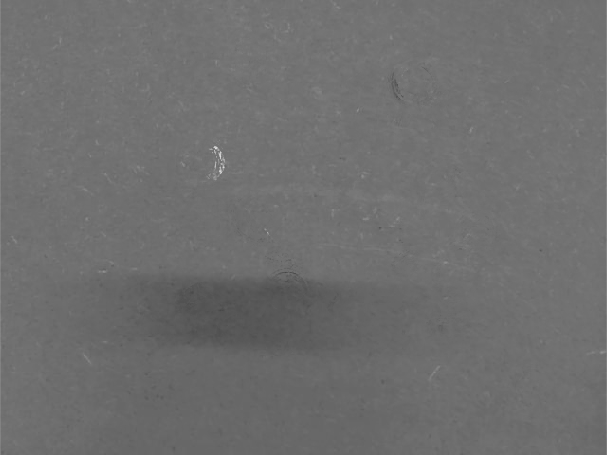
\includegraphics[width=\textwidth]{./img/bg_model/org_1.png}
    \caption{Background model without normalisation}
  \end{subfigure}
  \begin{subfigure}[b]{.45\textwidth}
    \centering
    
\includegraphics[width=\textwidth]{./img/bg_model/norm_1.png}
    \caption{Background model after normalisation}
  \end{subfigure}
  \caption{Background model generated from all 14 images.}
  \label{bg_model}
\end{figure}

Next, with objects scattered around randomly in the images, we find the median of all image pixels for each channel separately in order to reconstruct the background.
Our approach uses a neighbourhood of pixels for each pixel in the backgrund model. Hence, for a window of size 3, we have
$bg\_model_{r,c} = median(i_{r+1,c+1}, i_{r+1,c}, i_{r+1,c-1},
                          i_{r,c+1}, i_{r,c}, i_{r,c-1},
                          i_{r-1,c+1}, i_{r-1,c}, i_{r-1,c-1}) $.

The outcomes of the background (with and without normalisation) with different neighbourhood size = $1$, $3$, $5$ are shown in \autoref{montage_bg}. This appraoch requires large amount of memory and time to compute the background model. We find that although the images have subtle differences, the subimages we derieved in the later part of the pipeline is actually better.

\begin{figure}[!h]
  \centering
  \begin{subfigure}[t]{\textwidth}
    \centering
    \begin{subfigure}[t]{.3\textwidth} %% taking median
        \centering
        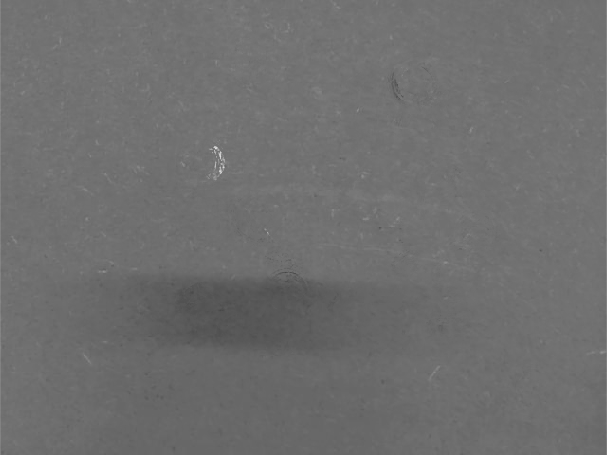
\includegraphics[width=\textwidth]{./img/bg_model/org_1.png}
    \end{subfigure}
    \begin{subfigure}[t]{.3\textwidth} %% window_size = 3
        \centering
        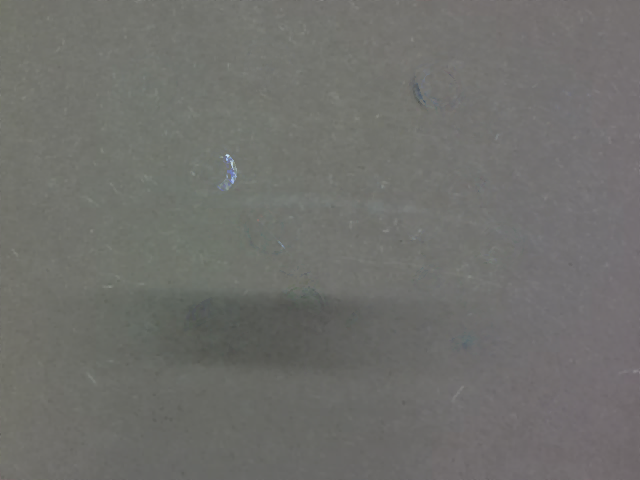
\includegraphics[width=\textwidth]{./img/bg_model/org_3.png}
    \end{subfigure}
    \begin{subfigure}[t]{.3\textwidth} %% window_size = 5
        \centering
        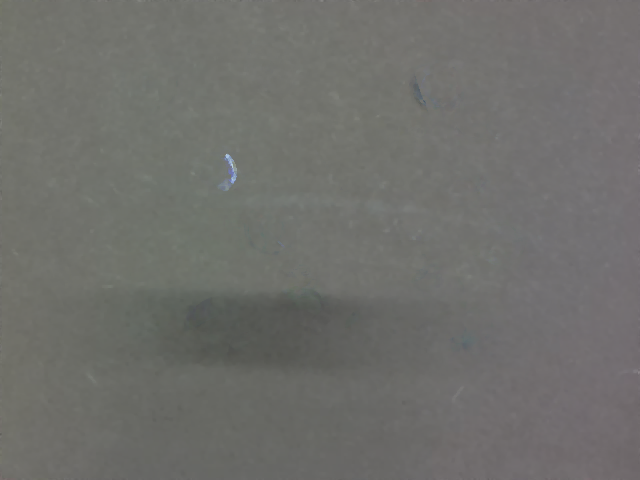
\includegraphics[width=\textwidth]{./img/bg_model/org_5.png}
    \end{subfigure}
  \end{subfigure} %% LOWER IMAGE - NORMALISED
  \begin{subfigure}[b]{\textwidth}
    \centering
    \begin{subfigure}[t]{.3\textwidth} %% taking median
        \centering
        
\includegraphics[width=\textwidth]{./img/bg_model/norm_1.png}
        \caption{Neighbouhood=1}
    \end{subfigure}
    \begin{subfigure}[t]{.3\textwidth} %% window_size = 3
        \centering
        
\includegraphics[width=\textwidth]{./img/bg_model/norm_3.png}
        \caption{Neighbourhood=3}
    \end{subfigure}
    \begin{subfigure}[t]{.3\textwidth} %% window_size = 5
        \centering
        
\includegraphics[width=\textwidth]{./img/bg_model/norm_5.png}
        \caption{Neighbourhood=5}
    \end{subfigure}
  \end{subfigure}
  \caption{Background extraction with different neighbourhood size.}
  \label{montage_bg}
\end{figure}


The sample images with their background removed is shown in \autoref{montage_data_bgremove}. This removal process: $img\_bg\_removed_{r,c}(R,G,B) = img_{r,c}(R,G,B) - bg\_model_{r,c}(R,G,B)$ , however, also inevitably reduce the intensity for the bottom half of each images, such that the objects are no longer salient. This is because the background we modelled have a lower intensity at the bottom, possibly due to presence of shadow in all 14 images.

An alternative approach we considered is to find the average of the neighbourhood. However, we did not materialise this, as the presence of high pixel intensity (such as in the presence of an object in the foreground) will distort the mean, giving an inaccurate representation of the background.

%% Can consider include historgram to show the effect?
% Nevertheless, the historgram  is still bimodal, which is essential for thresholding to be effective.
% ====================================================================== %

\subsubsection*{Segmentation}
After the background is removed, the objects are left in the image. Our next task is to extract these regions where the objects exists. We used \hyperlink{dothresh}{dothresh.m} on each image to:
\begin{enumerate}
  \item Find the histogram of the pixel intensity
  \item Find the threshold of the histogram - \texttt{thresh}
  \item Apply this threshold value to the image\\(i.e. $if$ $IMG_{i,j} \ge thresh$, $IMG_{r,c,chn} = 1,$ $else$ $ IMG_{r,c,chn} = 0$
  \item Produce a binary image, \texttt{BW}, using:$$BW_{r,c} = IMG_{r,c,R} || IMR_{r,c,G} || IMG_{r,c,B}$$
\end{enumerate}

The binary image indicates the existence of objects as 1 (white) and the background as 0 (black). \autoref{bin_image} are the binary images for the sample images.

%% INSERT IMAGE HERE!
\begin{figure}[!h]
  \centering
  \begin{subfigure}[b]{.3\textwidth}
    \centering
    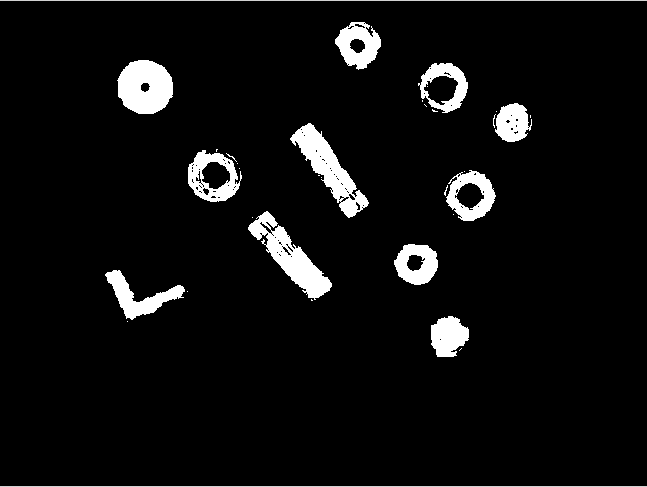
\includegraphics[width=\textwidth]{./img/srcimgs/normalised_img_bgremove/norm_bgrmv_thresh1.png}
  \end{subfigure}
  \begin{subfigure}[b]{.3\textwidth}
    \centering
    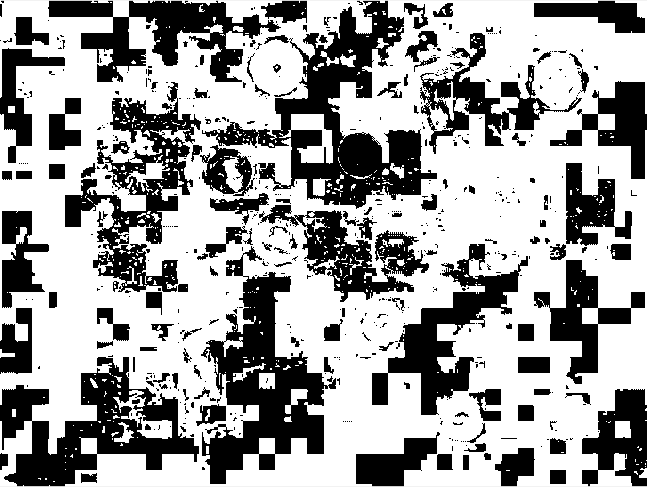
\includegraphics[width=\textwidth]{./img/srcimgs/normalised_img_bgremove/norm_bgrmv_thresh3.png}
  \end{subfigure}
  \begin{subfigure}[b]{.3\textwidth}
    \centering
    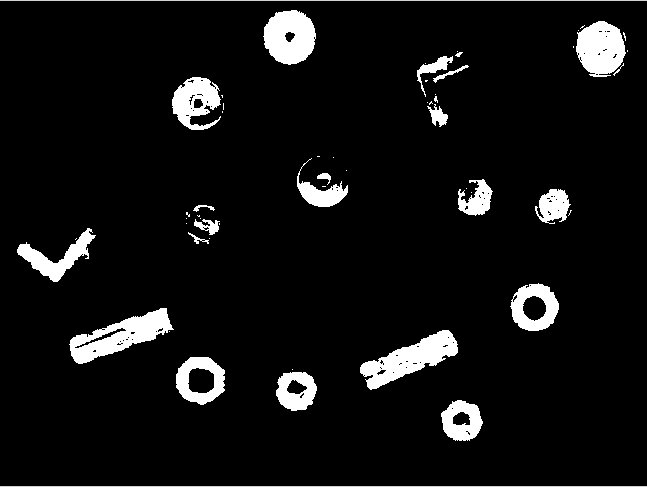
\includegraphics[width=\textwidth]{./img/srcimgs/normalised_img_bgremove/norm_bgrmv_thresh2.png}
  \end{subfigure}
  \caption{Black white images of normalised sample images with background removed.}
  \label{bin_image}
\end{figure}

\subsubsection*{Morphological Gradient Edge Detection}
Another model that we tried out, which performed better, is the morphological gradient edge detector (\hyperlink{gradmag}{gradmag\_edge.m}). Using a structuring element B (such as a disk with 5 pixel radius), we first find the  image A dilated with B and image A eroded with B separately. Then we subtract the two. Since the background is largely the same for both outcomes, the subtraction of each other will remove the background and retain the edges of each objects in the foreground.

We used \texttt{matalb} built in function to createa structuring element with disk radius of 3 pixels, and dilate and erode a given image. After the subtraction, we use the same thresholding function to get the binary image. The outcome of this operation is shown in \autoref{bin_morph}.

\begin{figure}[!h]
  \centering
  \begin{subfigure}[b]{.3\textwidth}
    \centering
    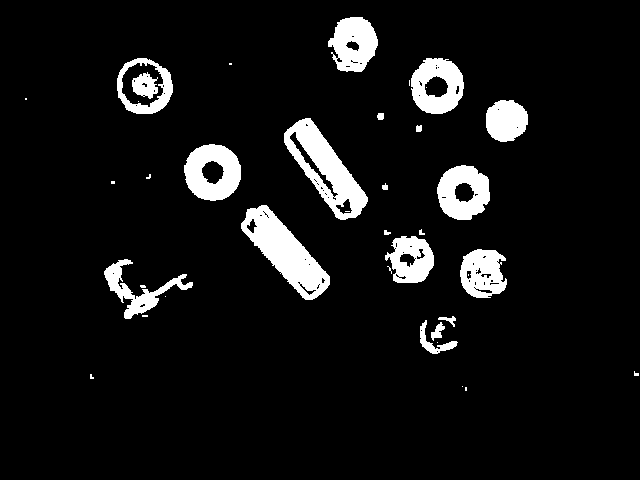
\includegraphics[width=\textwidth]{./img/srcimgs/morph_thresh/edges_morph_thresh1.png}
  \end{subfigure}
  \begin{subfigure}[b]{.3\textwidth}
    \centering
    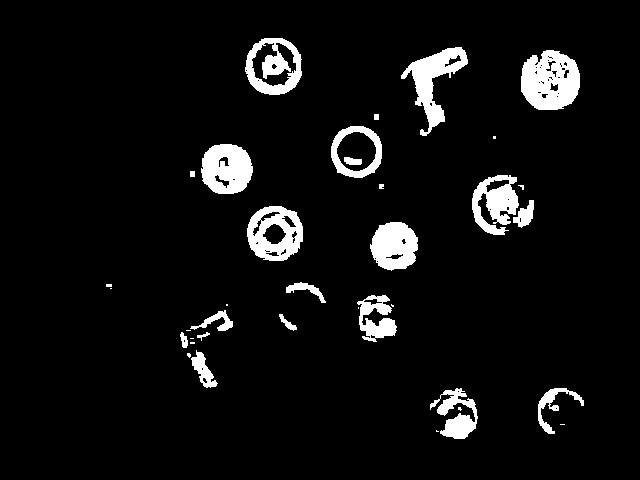
\includegraphics[width=\textwidth]{./img/srcimgs/morph_thresh/edges_morph_thresh3.png}
  \end{subfigure}
  \begin{subfigure}[b]{.3\textwidth}
    \centering
    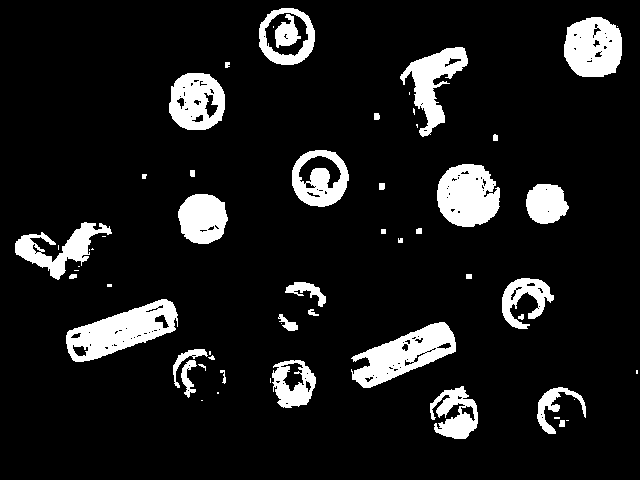
\includegraphics[width=\textwidth]{./img/srcimgs/morph_thresh/edges_morph_thresh2.png}
  \end{subfigure}
  \caption{Black white images of sample images after morphological gradient edge detection and thresholding. As the operator is background independent and does not require us to model the background first, the objects are more obvious now. And the centre sample image does not appaer to be a mess.}
  \label{bin_morph}
\end{figure}

The difference in result of extractiing images for this two different segmentation methods will be revealed in \hyperlink{result}{result section} later.

% ====================================================================== %
\subsubsection*{Filtering}
There are numerous filtering technique to make images better. One that we considered during the project is median filtering, and iterative median filtering. The aim is to preserve the edges while removing the noise in the background by find the median of the neighbourhood of the pixel. With the latter, the image undergoes any number of iteration until no visible change is observed. In our function, we utilised the \texttt{matlab} function \texttt{medfilt2}.

However, we realised that despite the changes in the edges, normalising an image is the main cause of a bad threshold. We are unable to find the threshold, as the gaussian smoothing operator in \texttt{findthresh} causes the bimodal peaks in the histogram of to become a unimodal peak. In this case, finding a useful threshold is futile.

\subsection{Feature Extraction}
The end product of the previous stage leaves us with an array of subimages. These subimages are black and white, such as those in \autoref{bw_subimg}. The output from this section is to have an array of features that uniquely defined each classes of objects defined above. We chose the following features:

\begin{enumerate}
  \item Area
  \item Perimeter
  \item Compactness
  \item Rectangularity
  \item Elongation
  \item Hu's invariant moments
  \item Complex invariant moments
  %       1) Area
%       2) Perimeter
%       3) compactness
%       4) rectangularity
%       5) elongation
%       6) hu moment invariant
%       7) complex invariant
\end{enumerate}

We later realised that the number of features is too large for our classifier, and casuse the covariance matrix to be almost singular. Although we regularised the matrix, we decided to remove Hu's invariant moments from the features, leaving us with 11 features to describe an object. Hence, for each subimages, there will be a feature vector of size 11.

\begin{figure}[!h]
  \centering
  \begin{subfigure}[b]{.2\textwidth}
    \centering
    
\includegraphics[width=\textwidth]{./img/srcimgs/bwimg-2.png}
  \end{subfigure}
  \begin{subfigure}[b]{.2\textwidth}
    \centering
    
\includegraphics[width=\textwidth]{./img/srcimgs/bwimg-3.png}
  \end{subfigure}
  \begin{subfigure}[b]{.2\textwidth}
    \centering
    
\includegraphics[width=\textwidth]{./img/srcimgs/bwimg-4.png}
  \end{subfigure}
  \begin{subfigure}[b]{.2\textwidth}
    \centering
    
\includegraphics[width=\textwidth]{./img/srcimgs/bwimg-5.png}
  \end{subfigure}
  \caption{Some subimages of the objects detected by \texttt{matlab} function \texttt{bwlabel}. It first find region where 1s are and give them a numeric label. Since pixel belonging to an object will come together, the numeric clsas will uniquely identify the object.}
  \label{bw_subimg}
\end{figure}

\subsection{Classification}
After extracting the features, \hyperlink{splitdata}{split\_data.m} will be called to split the dataset into the training set (\texttt{X\_train} and \texttt{y\_train}) and test set (\texttt{X\_test}) and \texttt{y\_test}). Then,
 \hyperlink{trainmultivarate}{trainmultivarate.m} will estimate the parameters based on the \texttt{X\_train} - the \texttt{prior}, \texttt{covariance} and \texttt{mean} for each class will be estimated.

 With these class parameters, the \hyperlink{gaussianDistr}{gaussianDistr.m} and \hyperlink{gaussianclf}{gaussian\_clf.m} will be called to estimate the posterior probability for each object in \texttt{X\_test}.

 \subsubsection*{Linear Discriminant - average covariance for all classes}
We consider the use case of a Linear Discriminant function. Howwever, on second though, the idea that all objects (classes) having the same covariance does not quite make sense. Since the features describe the data, the covariance of the feature set should be unique to all the object.

The classification step outputs the confusion matrix for the data, such as this one when the multivarate classifier is trained with 75 percent of the data and 25 percent of it for the test data.

\begin{verbatim}
  ========================================================
>> trainmultivarate
Done!

The confusion matrix is:
(rows = actual class; columns = predicted class)
     0     0     0     0     0     0     0     0     0     0
     0     0     0     0     0     0     0     0     0     0
     0     3     0     0     0     0     0     0     0     0
     0     0     0     2     1     0     0     0     0     0
     0     0     0     0     1     0     0     0     0     0
     0     0     0     0     0     1     0     1     0     0
     0     0     0     0     0     0     1     0     0     0
     0     0     0     0     0     0     0     2     2     0
     0     0     0     0     0     0     0     0     1     0
     0     1     0     0     1     0     0     0     0     2

The classification results for each class are:
   (FN    FP    TP   TN)
     0     0     0    19
     0     4     0    15
     3     0     0    16
     1     0     2    16
     0     2     1    16
     1     0     1    17
     0     0     1    18
     2     1     2    14
     0     2     1    16
     2     0     2    15
========================================================
Summary:
Classification using full gaussian model
Number Incorrect = 18
Number Correct = 10
Number of classes = 10
Accuracy = 0.526316 percent
========================================================
\end{verbatim}

\begin{figure}[!h]
  \centering
  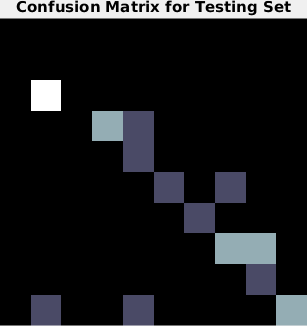
\includegraphics[width=\textwidth]{./img/srcimgs/cm_01.png}
  \caption{Confusion Matrix, with rows representing actual class and columns representing predicted class. A brighter white indicates a higher number of true positive. The class 1 (1 pound coin) have no boxes lit up, signifying that this test set does not have any 1 pound coin in it}
\end{figure}


\end{document}
